\chapter{Lecture three: Structure}
\begin{comment}
\section{Problem domain analysis}

\subsection{Results}
Class diagram and behavioural patterns, or state-change diagrams for each class. 
This could possibly be done in UML.


\subsection{Key concepts}
The problem domain is the part of a context that is administrated, monitored, or controlled by a system. Examples of problem domains:
\begin{itemize}
    \item Students in a education institution
    \item Employees in a company
    \item Items in a warehouse
    \item Customers in a hair salon
    \item Movies available for streaming
\end{itemize}


\subsection{Classes: Results}

\begin{table}[h]
\centering
\begin{tabular}{l|l|l|l|l|l|l|l|}
\cline{2-8}
 & reserved & cancel & treated & employed & resigned & graduated & agreed \\ \hline
\multicolumn{1}{|l|}{Customer} & \checkmark & \checkmark & \checkmark &  &  &  &  \\ \hline
\multicolumn{1}{|l|}{Assistant} & \checkmark & \checkmark &  & \checkmark & \checkmark &  & \checkmark \\ \hline
\multicolumn{1}{|l|}{Apprentice} &  &  &  & \checkmark & \checkmark & \checkmark & \checkmark \\ \hline
\multicolumn{1}{|l|}{Appointment} & \checkmark & \checkmark & \checkmark &  &  &  &  \\ \hline
\multicolumn{1}{|l|}{Plan} & \checkmark &  &  &  &  &  & \checkmark \\ \hline
\end{tabular}
\caption{Event table for hair salon}
\end{table}

Shows major classes and events in the problem domain. The classes are often listed horizontally, but depends on number of each.

\section{Classifying objects and events in the problem domain}
Abstract and classify phenomena in the problem domain into objects and events within the requirements mentioned in earlier sections.

\section{Key concepts: Event}
An \textbf{event} is an instantaneous incident involving one or more objects. These are \textbf{atomic, instantaneous, common to several objects, and unique in name.}

Examples from IKEA:
\begin{itemize}
    \item Item received from producer
    \item Item stored in warehouse
    \item Item selected by customer
    \item Item picked in warehouse - OK?
    \item Item sold
\end{itemize}


\section{Classes: Summary}
\begin{table}[h]
\centering
\begin{tabular}{|l|l|}
\hline
Purpose & To select the elements of a problem-domain model. \\ \hline
Concepts & \begin{tabular}[c]{@{}l@{}}Object: An entity with identity, state, and behaviour.\\ Class: A description of a collection of objects sharing structure, behavioural pattern, and attributes.\\ Event: An instantaneous incident involving one or more objects.\end{tabular} \\ \hline
Principles & \begin{tabular}[c]{@{}l@{}}Classify objects in the problem domain.\\ Charaterise objects through their events.\\ Have an open mind, but select critically.\end{tabular} \\ \hline
Results & An event table with classes and related events. \\ \hline
\end{tabular}
\end{table}
\end{comment}

%old shit above
\section{Structure}
\subsection{Result}
This activity results in a class diagram.
\begin{figure}[H]
    \centering
    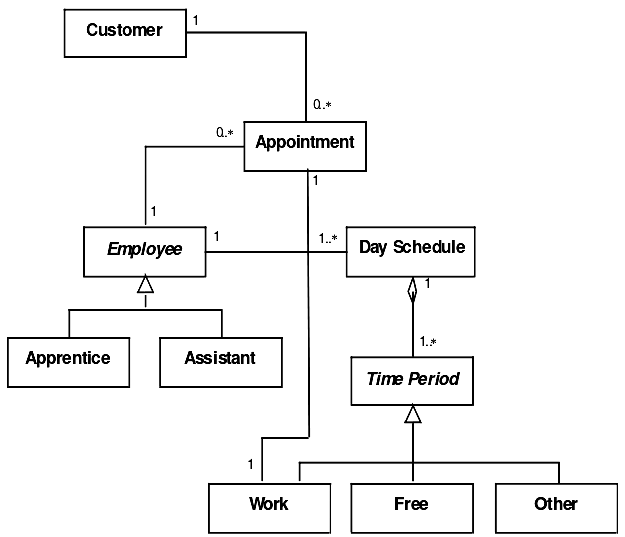
\includegraphics[width=.6\textwidth]{figures/classdiagram.png}
\end{figure}
\subsection{Key concepts}
\subsubsection{Generalisation}
Generalisation: A general class (the super class) describes properties common to a group of specialised classes (the subclasses)
Object oriented, as in a passenger car can both be a taxi and a private car. This is essentially \textbf{is-a} relations, e.g. \textit{a taxi \textbf{is-a} passenger car}. 

\begin{figure}[H]
    \centering
    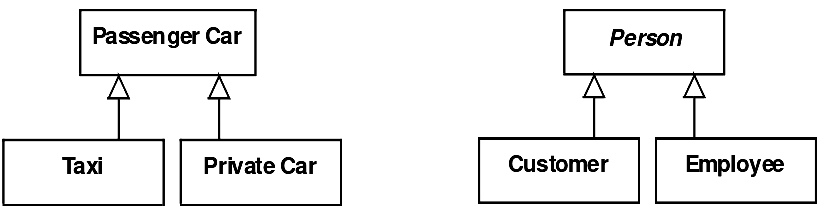
\includegraphics[scale=1.5]{figures/generalisation.png}
\end{figure}

Furthermore, there's generalisation, specialisation, and abstract classes. Abstract classes are denoted by \textit{italics}.

\subsubsection{Cluster}
A collection of related classes
\begin{figure}[H]
    \centering
    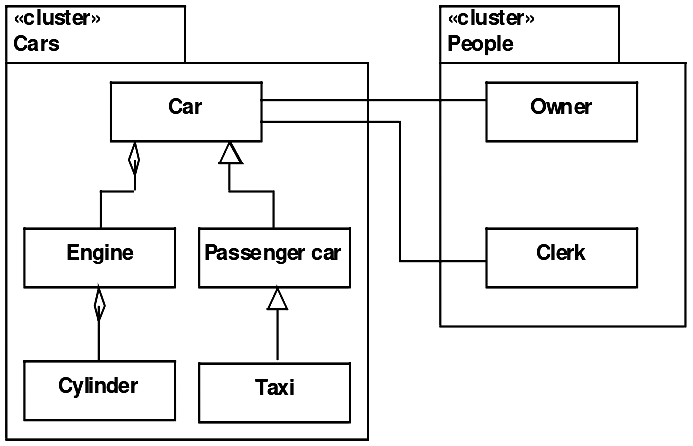
\includegraphics[scale=1.5]{figures/cluster.png}
\end{figure}

\subsubsection{Aggregation}
Aggregation: A superior object (the whole) consists of a number of inferior objects (the parts). The aggregation structure drawn with a line, and a rhomb at (the whole) class.
Physical aggregation (unusual), relations alike \textbf{has-a} or \textbf{owns-a}, these are more common. Usually on different, conceptual, levels. Typical aggregations; whole - part, container - contents, and union - member.

\begin{figure}[H]
    \centering
    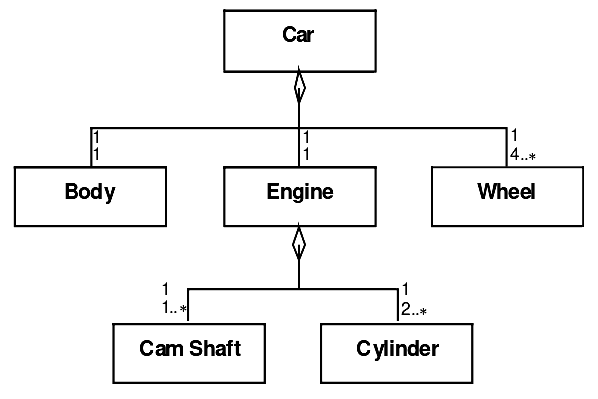
\includegraphics[scale=1.5]{figures/aggregation.png}
\end{figure}

\subsubsection{Association}
Association: A meaningful relation between a number of objects. This is often used when aggregation would imply a too strong relation. Linguistically, express association with "knows" or "associated-with".
Relations, usually a loose (non-defining) relation, usually on the same \textit{level}, and these can be named (but this is often because a class is missing, so instead of naming the association, we can introduce that class). 
\begin{figure}[H]
    \centering
    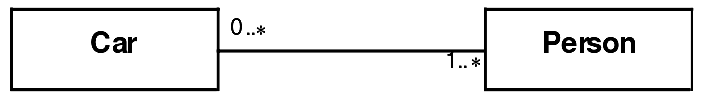
\includegraphics[scale=1.5]{figures/association.png}
\end{figure}

\subsection{Activities}
\begin{figure}[H]
    \centering
    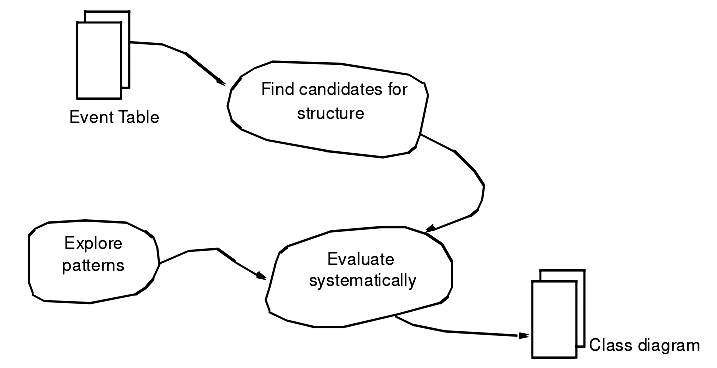
\includegraphics[scale=1.5]{figures/structureactivity.png}
\end{figure}

\subsection{Evaluate systematically}
\begin{itemize}
    \item Structures must be used correctly
    \begin{itemize}
        \item Generalisation versus aggregation (\textit{is-a / has-a})
        \item Aggregation versus association (page 87 in \ad)
    \end{itemize}
    \item Structures must be conceptually true
    \begin{itemize}
        \item Names, concepts, and structures reflect the user's understanding
        \item Especially for the prospective user
    \end{itemize}
    \item Structures must be simple
    \begin{itemize}
        \item Especially at the top levels
        \item Avoid unnecessary generalisations and aggregations
        \item Avoid objects changing class
        \item Check against the system definition
    \end{itemize}
\end{itemize}

\section{Discuss hair salon class diagram}
\begin{figure}[H]
    \centering
    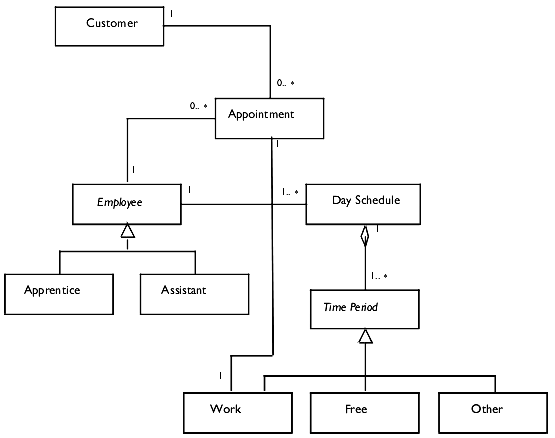
\includegraphics[width=.75\textwidth]{figures/hairsalondiscussion.png}
\end{figure}

Customer and appointment is a candidate for aggregation, as it satisfied properties specified on page 87.

\noindent The following were found during lecture discussion:
\begin{itemize}
    \item Customer - Appointment: Aggregation from Customer
    \item Appointment - Employee: OK
    \item Employee - Day Schedule: Aggregation from Employee
    \item Time Period specialisations: Different solution, e.g. remove the tree specialisations
\end{itemize}

\subsection{Summary}
\begin{figure}[H]
    \centering
    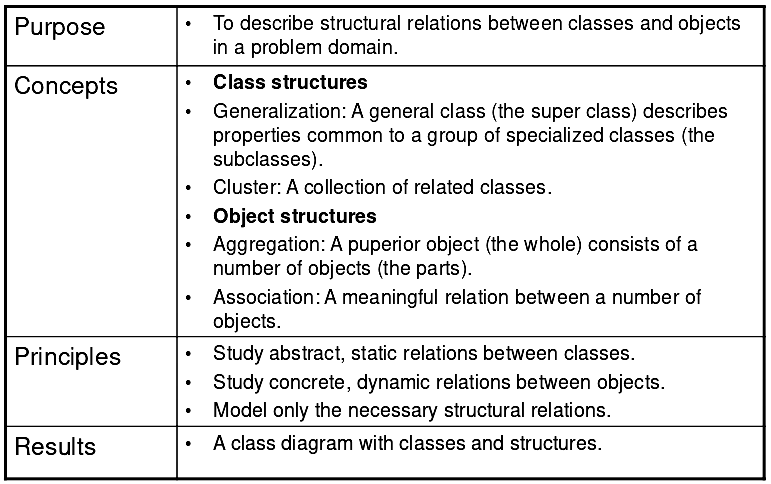
\includegraphics[scale=2]{figures/structuresummary.png}
\end{figure}

\section{Example with a streaming service}\label{structure:streamingservice}
\begin{itemize}
    \item[] \textit{Functionality:} Register the movies the customers see and the songs they listen to, and support payment by customers for their consumption of movies and songs
    \item[] \textit{Application domain:} Will be used by the administrative personnel that is employed by the organisation that provides the streaming service
    \item[] \textit{Conditions:} Developed for the administrative personnel
    \item[] \textit{Technology:} PC platform with typical tools
    \item[] \textit{Objects:} Customer, Movie, Song
    \item[] \textit{Responsibility:} Registration, administration, and payment of customers' consumption
\end{itemize}

An initial class diagram for this FACTOR:
\begin{figure}[H]
    \centering
    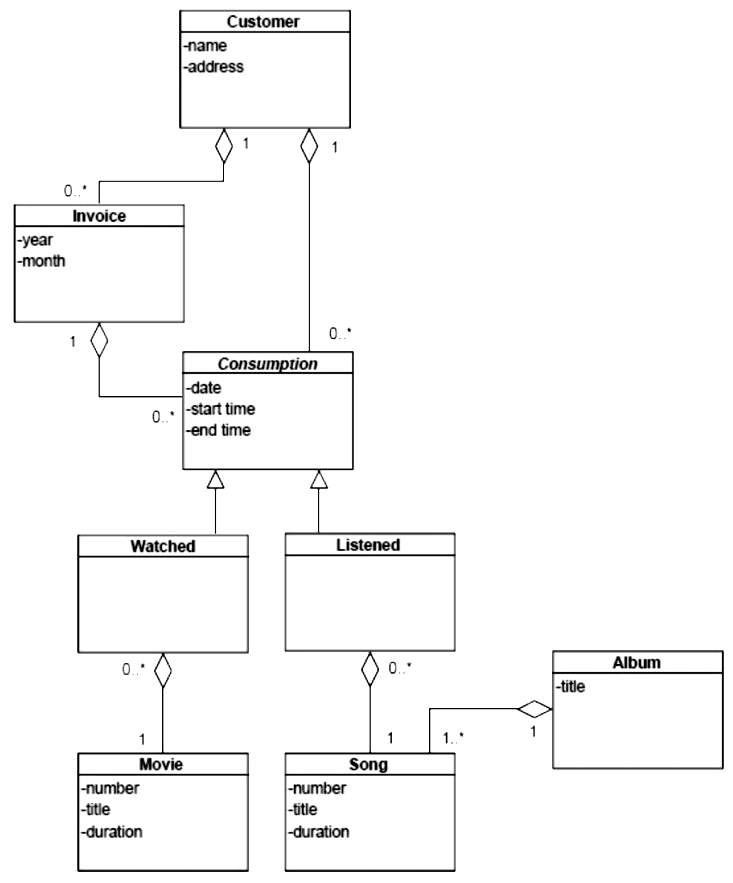
\includegraphics[width=.5\textwidth]{figures/prelimstreamclassdiagram.png}
\end{figure}

\section{Patterns}
\subsection{Role pattern}
A person can have different roles. The roles of a person change dynamically over time. Here employees and customers are generalised into persons. A person then aggregates one or more roles. If the roles have nothing in common, we use a simplified pattern without the role class, with the employee role and customer role directly aggregates to person.

\begin{figure}[H]
    \centering
    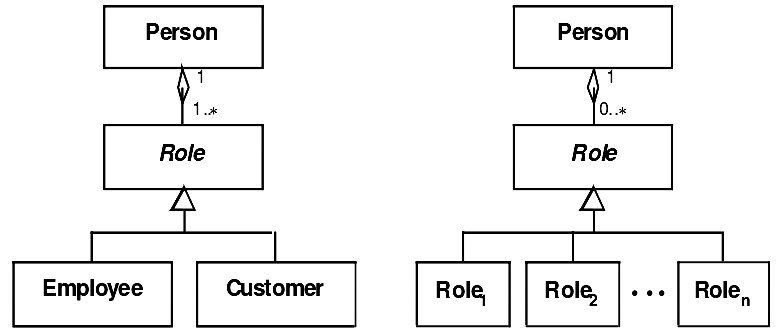
\includegraphics[width=.5\textwidth]{figures/rolepattern.png}
\end{figure}

\subsection{Relation pattern}
The purpose of the pattern is to relate two parties to each other. Two variations; In the first, both of the related parties aggregate the relation object. This indicates that they both own the relation. Second variation is both parties connect to the relation with association. This indicates a loose relation.

\begin{figure}[H]
    \centering
    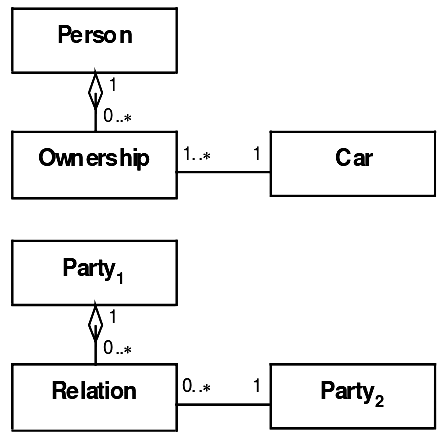
\includegraphics[width=.35\textwidth]{figures/relationpattern.png}
\end{figure}

\subsection{Hierarchy pattern}
When using this pattern, we must decide what the elements are and how many levels of hierarchy to organise them in. In chapter 19, an advanced application of this pattern is shown in the "Program" cluster of the conference planning system. A useful variation on this pattern, is where objects on one level, can belong to several objects on the level above. 

\begin{figure}[H]
    \centering
    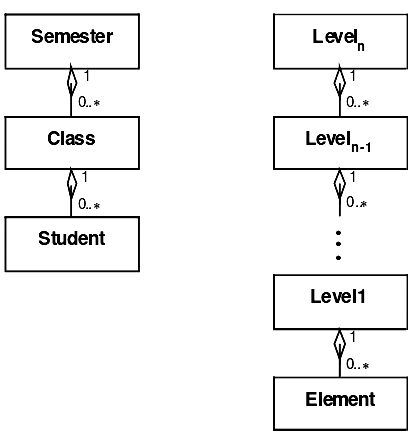
\includegraphics[width=.4\textwidth]{figures/hierachypattern.png}
\end{figure}

\subsection{Item-descriptor pattern}
Properties of objects from one class (items) are described in an object from another class (descriptor). An object from the overall class "Descriptor" defines specific properties shared by all the related objects from the "Item" class. This pattern is useful in systems that administrate different kind of descriptions, such as contracts, insurance policies and so on.

\begin{figure}[H]
    \centering
    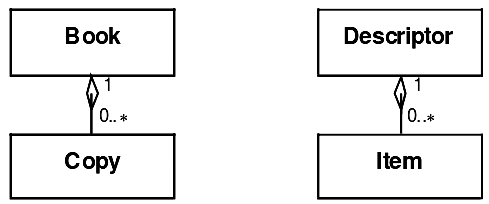
\includegraphics[width=.4\textwidth]{figures/itemdescriptorpattern.png}
\end{figure}

\section{Challenges}
\begin{itemize}
    \item Selecting the right structure is difficult
    \begin{itemize}
        \item Try them out one-by-one for each pair of classes
        \item Use the criteria to select the most correct structure.
    \end{itemize}
    \item It is very easy to include too many structures
    \begin{itemize}
        \item Try to simulate functions and see if you can get to the relevant objects.
    \end{itemize}
\end{itemize}

\noindent A good test is to try out functions and notice if any objects are not relevant.

\section{Principles}
\subsection{Study abstract, static relations between classes}
We use generalisation and cluster structures to describe static, conceptual relations between classes. Generalisation structures express different levels of abstraction in our model, while we use clusters to achieve clarity.

\subsection{Study concrete, dynamic relations between objects}
We use aggregation and association structures to describe dynamic, concrete relations between objects. Aggregation structures describe superior objects as consisting of or containing subobjects, while association structures describe other meaningful relations between objects.

\subsection{Model only the necessary structural relations}
The model should describe only the structural relations that are necessary to satisfy the system definition. In general, the model should focus on the important aspects and contain a minimal number of structural relations. 

\section{Exercises for lecture three}
\begin{itemize}
    \item Find candidates for structural relations between the classes in your event table - \textit{do this in pairs}
    \item Explore if any of the patterns are relevant to your case - \textit{do this for each class}
    \item Make a class diagram
    \item Look for opportunities to simplify and extend the class diagram
\end{itemize}
\subsection{Quiz}
92\% correct over 8 minutes.

Object structure and role-patterns had errors in the quiz.